\documentclass{article}
\usepackage[T1]{fontenc}
\usepackage{lmodern}
\usepackage{graphicx}
\usepackage{amsmath,amssymb}
\usepackage[a4paper,margin=2cm]{geometry}
\usepackage[absolute,overlay]{textpos}
\setlength{\TPHorizModule}{1mm}
\setlength{\TPVertModule}{1mm}
\usepackage[indonesian]{babel}
\usepackage{hyperref}
\setlength{\emergencystretch}{2em}
% unit: Halaman 44

\begin{document}

% === Halaman 44 (llm) ===

# Program utama

#Alice membangkitkan kunci publik dan kunci privatnya\nprint("\nKUNCI PUBLIK DAN KUNCI PRIVAT ALICE:")\nPembangkitanKunciRSA('kunci\_publik\_Alice.pem', 'kunci\_privat\_Alice.pem')

\vspace{169.29mm}

#Bob membangkitkan kunci publik dan kunci privatnya\nprint("\nKUNCI PUBLIK DAN KUNCI PRIVAT BOB:")\nPembangkitanKunciRSA("kunci\_publik\_Bob.pem", "kunci\_privat\_Bob.pem")

#Bob mengirim pesan kepada Alice\npesan = input("\nBob, ketikkan pesan teks buat Alice: ")

#Bob mengenkripsi pesan dengan menggunakan kunci publik Alice\nciphertext = encrypt\_message(pesan, 'kunci\_publik\_Alice.pem')\nprint("\nCiphertext (dari Bob):", ciphertext.hex())

#Alice mendekripsi ciphertext dari Bob menggunakab kunci privatnya sendiri\n(kunci privat Alice)\ndecrypted\_message = decrypt\_message(ciphertext, 'kunci\_privat\_Alice.pem')\nprint("\nPesan setelah dekripsi oleh Alice:", decrypted\_message)

% deskripsi: Screenshot potongan kode program Python yang mengilustrasikan proses enkripsi dan dekripsi menggunakan algoritma RSA antara dua pengguna, Alice dan Bob.
% bbox normalisasi: [0.0900, 0.3000, 0.9300, 0.8700]
\begin{textblock*}{176.40mm}(18.90mm,89.10mm)
\noindent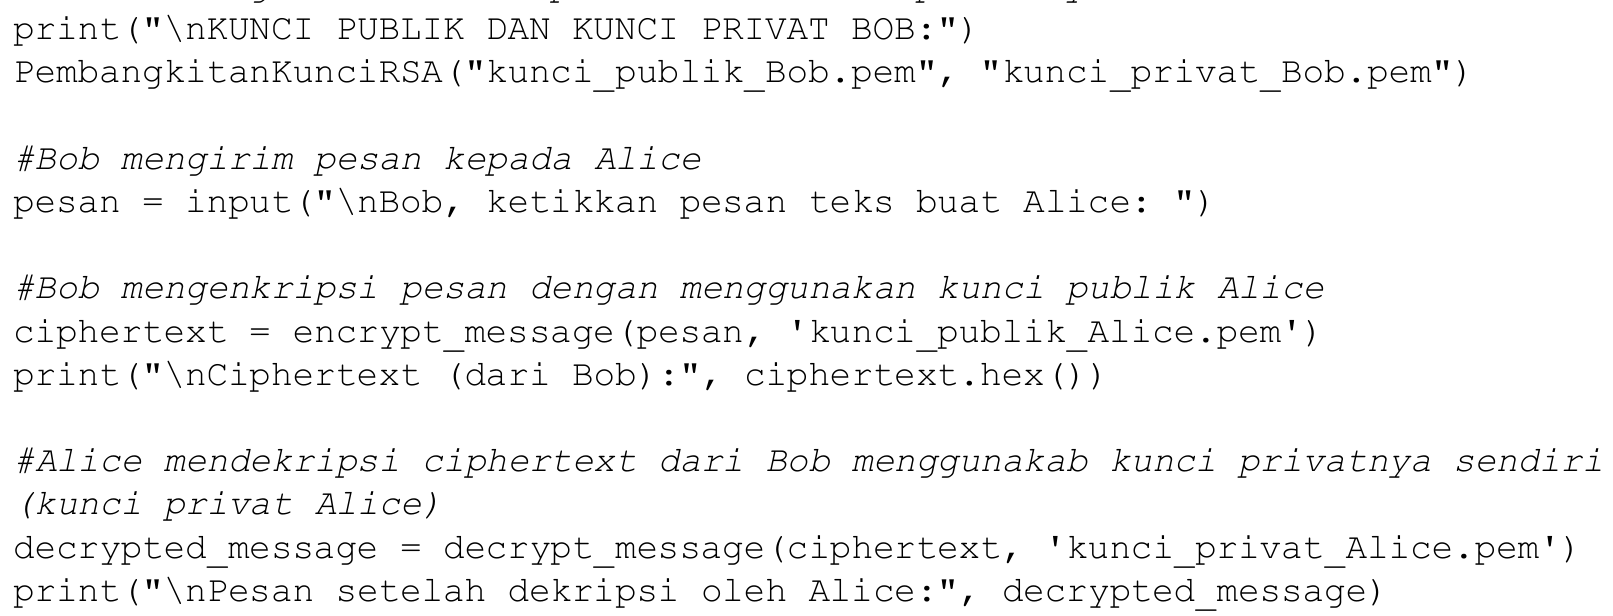
\includegraphics[width=176.40mm,height=169.29mm]{../../images/llm/page_044_img_01.png}%
\end{textblock*}

\end{document}
